% Copyright 2004 by Till Tantau <tantau@users.sourceforge.net>.
%
% In principle, this file can be redistributed and/or modified under
% the terms of the GNU Public License, version 2.
%
% However, this file is supposed to be a template to be modified
% for your own needs. For this reason, if you use this file as a
% template and not specifically distribute it as part of a another
% package/program, I grant the extra permission to freely copy and
% modify this file as you see fit and even to delete this copyright
% notice. 

\documentclass{beamer}
\usepackage[utf8]{inputenc}
% There are many different themes available for Beamer. A comprehensive
% list with examples is given here:
% http://deic.uab.es/~iblanes/beamer_gallery/index_by_theme.html
% You can uncomment the themes below if you would like to use a different
% one:
%\usetheme{AnnArbor}
%\usetheme{Antibes}
%\usetheme{Bergen}
%\usetheme{Berkeley}
%\usetheme{Berlin}
%\usetheme{Boadilla}
%\usetheme{boxes}
\usetheme{CambridgeUS}
%\usetheme{Copenhagen}
%\usetheme{Darmstadt}
%\usetheme{default}
%\usetheme{Frankfurt}
%\usetheme{Goettingen}
%\usetheme{Hannover}
%\usetheme{Ilmenau}
%\usetheme{JuanLesPins}
%\usetheme{Luebeck}
%\usetheme{Madrid}
%\usetheme{Malmoe}
%\usetheme{Marburg}
%\usetheme{Montpellier}
%\usetheme{PaloAlto}
%\usetheme{Pittsburgh}
%\usetheme{Rochester}
%\usetheme{Singapore}
%\usetheme{Szeged}
%\usetheme{Warsaw}

\usepackage{natbib}
\usepackage{apalike}
\usepackage{longtable}
\usepackage{tikz}
\usepackage{hyperref}

% Let's get started
\begin{document}

\title{Ethics in Applied AI}

% A subtitle is optional and this may be deleted
\subtitle{Ethics in Applied Artificial Intelligence\\
POLS200 - Ethics in Social Sciences}

\author{YASIN KUTUK, Ph.D.*}
% - Give the names in the same order as the appear in the paper.
% - Use the \inst{?} command only if the authors have different
%   affiliation.

\institute[AU] % (optional, but mostly needed)
{  \inst{*}%
  Department of Economics - Altınbaş Univ. \\

}
% - Use the \inst command only if there are several affiliations.
% - Keep it simple, no one is interested in your street address.



\date{2022-02-03}
% - Either use conference name or its abbreviation.
% - Not really informative to the audience, more for people (including
%   yourself) who are reading the slides online

%\begin{figure}
%\includegraphics[scale=0.025]{./img/itu-logo.png}
%\end{figure}

\subject{Course Presentation}
% This is only inserted into the PDF information catalog. Can be left
% out. 

% If you have a file called "university-logo-filename.xxx", where xxx
% is a graphic format that can be processed by latex or pdflatex,
% resp., then you can add a logo as follows:

% \pgfdeclareimage[height=0.5cm]{university-logo}{university-logo-filename}
% \logo{\pgfuseimage{university-logo}}

% Delete this, if you do not want the table of contents to pop up at
% the beginning of each subsection:
\AtBeginSubsection[]
{
  \begin{frame}<beamer>{Outline}
    \tableofcontents[currentsection,currentsubsection]
  \end{frame}
}




\begin{frame}
  \titlepage
\end{frame}





\begin{frame}{Outline}
  \tableofcontents
  % You might wish to add the option [pausesections]
\end{frame}

% Section and subsections will appear in the presentation overview
% and table of contents.



%\section{Outline}


\section{What is AI?}
\begin{frame}{Definition of AI}
\textbf{Artificial Intelligence (AI)} refers to systems that display intelligent behaviour by analysing their environment and taking actions – with some degree of autonomy – to achieve specific goals \citep{ec2011communication}.
%\\~\
\end{frame}

\begin{frame}{How do we define intelligence?}
A straightforward definition is that intelligent behaviour is 'doing the right thing at the right time'.
\\~\
\cite{legg2007collection} - informal definitions. Intelligence is
\begin{itemize}
\item a property that an individual agent has as it interacts with its environment or environments. 
\item related to the agent's ability to succeed or profit with respect to some goal or objective.
\item depends on how able that agent is to adapt to different objectives and environments.
\end{itemize}
\end{frame}

\subsection{Artificial Intelligence}
\begin{frame}{Narrow-AI?}
All present-day AIs and robots are examples of what we refer to as \textbf{'narrow' AI}: a term that reflects that fact that current AIs and robots are typically only capable of undertaking one specialised task.
\end{frame}


\begin{frame}{Artificial General Intelligence}
A long-term goal of AI and robotics research is so-called \textbf{artificial general intelligence (AGI)} which would be comparable to human intelligence.
\end{frame}

\subsection{Applied Artificial Intelligence}
\begin{frame}{Machine Learning (ML)}
\textbf{Machine learning} is the term used for AIs which are capable of learning or, in the case of robots, adapting to their environment.
\end{frame}

\begin{frame}{Artificial Neural Networks (ANNs)}
Supervised learning systems generally make use of \textbf{Artificial Neural Networks (ANNs)}, which are trained by presenting the ANN with inputs (for instance, images of animals) each of which is tagged (by humans) with an output (i.e. giraffe, lion, gorilla).
\end{frame}

\begin{frame}{Deep Learning (DL)}
The term \textbf{deep learning} simply refers to (typically) supervised machine learning systems with large (i.e. many-layered) ANNs and large training data sets.
\begin{figure}
\centering
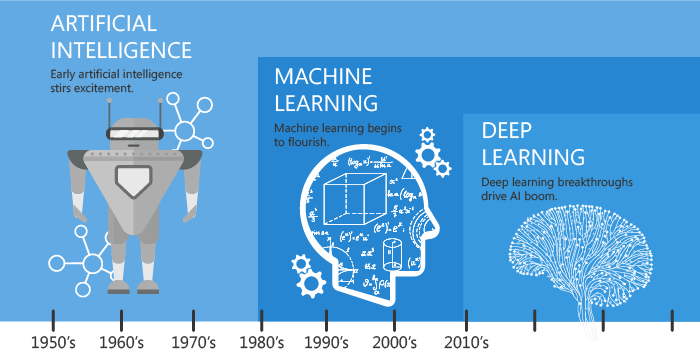
\includegraphics[scale=0.35]{ai-ml-dl-2.png}\\
\floatfoot{\footnotesize source: medium.com@alanb\_73111}
\end{figure}
It is important to note the terms AI and ML/DL are not synonymous. Many highly capable AIs and robots do not make use of ML.
\end{frame}



\begin{frame}{Ethics and its Relation to Applied AI}
Ethics are moral principles that govern a person's behaviour or the conduct of an activity. As a practical example, one ethical principle is to treat everyone with respect. Philosophers have debated ethics for many centuries, and there are various well-known principles, perhaps one of the most famous being Kant's categorical imperative 'act as you would want all other people to act towards all other people' \citep{kant2008groundwork}.
\end{frame}




\section{Ethical Impacts of Applied AI}

\begin{frame}{Ethical Impacts of Applied AI}
Within the last 5 years AI ethics has shifted from an academic concern to a matter for political as well 
as public debate.

\\~\

The increasing ubiquity of smart phones and the AI-driven applications that many  of us now rely on every day, the fact that AI is increasingly impacting all sectors (including industry,  healthcare, policing & the judiciary, transport, finance and leisure), as well as the seeming prospect  of an AI 'arms race', has prompted an extraordinary number of national and international initiatives, from NGOs, academic and industrial groupings, professional bodies and governments \citep{bird2020ethics}.
\end{frame}

\subsection{Impact on Society}

\begin{frame}{The labour market}
\begin{itemize}
    \item Automation has often substituted for human labour in the short term, but has led to the creation of jobs in the long term \citep{david2015there}.
    \item Robotics added an estimated 0.4 percentage \citep{graetz2015robots}.
    \item Vast increases in income inequality, large numbers of unemployable people, and breakdowns in the social order 
\citep{smith2014ai}.
\end{itemize}


\end{frame}


\begin{frame}{Inequality}
\begin{itemize}
    \item Concentration of power among elites \citep{nemitz2018constitutional}.
\end{itemize}
\end{frame}

\begin{frame}{Privacy, human rights and dignity}
\begin{itemize}
    \item Intelligent Personal Assistants
    \item Big Data
    \item Facial Recognition, Data Mining
    \item Brexit Case \citep{cadwalladr2017revealed}.
\end{itemize}
\end{frame}


\begin{frame}{Bias}
\begin{itemize}
    \item AI is created by humans, which means it can be susceptible to bias.
    \item COMPAS Case \citep{kirchner2016machine}.
\end{itemize}
\end{frame}

\begin{frame}{Democracy}
\begin{itemize}
    \item Fake news and social media \citep{gorodnichenko2021social}.
    \item At least 28 countries — including both authoritarian states and democracies — employ 'cyber troops' \citep{bradshaw2017troops}.
    \item The end of democracies? \citep{bartlett2018people}.
\end{itemize}
\end{frame}



\subsection{Impact on Financial System}

\begin{frame}{Impact on Financial System}
\begin{itemize}
    \item Market manipulation \citep{spatt2014security}.
    \item Collusion \citep{ezrachi2017two}.
    \item Accountability \citep{wellman2017ethical}.
\end{itemize}
\end{frame}


\subsection{Impact on Legal System}

\begin{frame}{Impact on Legal System}
The most important near-term legal question associated with AI is who or what should be liable for tortious, criminal, and contractual misconduct involving AI and under what conditions.
\end{frame}

\begin{frame}{Criminal law}
\begin{itemize}
    \item Liability: bankruptcy of the corporation? \citep{pagallo2018apples}
    \item Commerce, financial markets and insolvency \citep{farmer2013ecological}.
    \item Offences Against the Person, Individual Rights \citep{citron2018deep}.
\end{itemize}
\end{frame}

\begin{frame}{Tort law}
\begin{itemize}
    \item Tort law covers situations where one person's behaviour causes injury, suffering, unfair loss, or harm 
to another person.
    \item Two purposes: compensation, deterrioration.
\end{itemize}
\end{frame}


\subsection{Impact on Environment and the Planet}

\begin{frame}{Use of natural resources}
\begin{itemize}
    \item Exploitation of raw resources.
    \item Mining and misuse of metals \citep{khakurel2018rise}.
\end{itemize}
\end{frame}

\begin{frame}{Pollution and wast}
\begin{itemize}
    \item Electronic waste.
    \item Sustainability \citep{guiltinan2009creative}.
\end{itemize}
\end{frame}

\begin{frame}{Energy concerns}
\begin{itemize}
    \item Supply problems.
    \item Carboon footprints \citep{strubell2019energy}.
\end{itemize}
\end{frame}

\begin{frame}{Ways AI could help the planet}
\begin{itemize}
    \item Reducing gas emmissions \citep{iglinski2017analysis}.
    \item Make biodiversification efficient.
\end{itemize}
\end{frame}


\subsection{Impact on Trust}

\begin{frame}{Impact on Trust}
\begin{itemize}
    \item The overwhelming consensus amongst the research community is that trust in AI can only be 
attained by fairness, transparency, accountability and regulation.
    \item How much control we want to exert over AI machines, and if, for example we want to always 
maintain a human-in the loop, or give systems more autonomy.
\end{itemize}
\end{frame}



\begin{frame}{Fairness}
Four requirements: \cite{corbett2017algorithmic}
\begin{itemize}
    \item Statistical parity,
    \item Conditional statistical parity,
    \item Predictive equality,
    \item Calibration.
\end{itemize}
\end{frame}

\begin{frame}{Transparency}
\begin{itemize}
    \item Autopiloting.
    \item Being a \textbf{black box}, \cite{kroll2018fallacy}.
    \item Explainable systems.
    \item Intentional understanding.
\end{itemize}
\end{frame}


\begin{frame}{Accountability}
\begin{itemize}
    \item Tesla Model S, Uber cases.
    \item Regulations, \citep{winfield2018ethical}.
\end{itemize}
\end{frame}

\begin{frame}{Control}
\begin{itemize}
    \item Jumping to Superintelligence?
    \item Human in the loop (HITL) \citep{rahwan2018society}.
    \item Hell Yeah: THE BIG RED BUTTON \citep{orseau2016safely}.
\end{itemize}
\end{frame}


\section{Ethical AI}
\begin{frame}{Final Thoughts}
\begin{itemize}
    \item We need industrialisation and productivity.
    \item Make research.
    \item Re-trainable programs.
    \item Collaboration (transparent).
    \item Inclusive Social Development.
    \item Responsibility.
\end{itemize}
\end{frame}



\section{References}

\begin{frame}[allowframebreaks]
\footnotesize
        \frametitle{References}
        \bibliographystyle{apalike}
        \bibliography{refs.bib}
\normalsize
\end{frame}

\begin{frame} {Thanks}

\begin{center}
for your convenience...\\
\\~\
\\~\
\href{mailto:yasin.kutuk@altinbas.edu.tr}{yasin.kutuk@altinbas.edu.tr}\\
\\~\
\\~\
Google Scholar Profile: \href{https://scholar.google.com.tr/citations?user=Cj_erekAAAAJ&hl=tr&oi=ao}{Link}
\\~\
\\~\
Github Profile \footnote{\tiny includes source code of this presentation and its compiled PDF.}: \href{https://github.com/yasinkutuk/}{Link}
\end{center}
\end{frame}




\end{document}



